% http://tex.stackexchange.com/questions/11866/compile-a-latex-document-into-a-png-image-thats-as-short-as-possible#11880
%http://tex.stackexchange.com/questions/152247/best-practice-to-include-standalone-precompiled-graphics
\documentclass[border=1pt]{standalone}
\usepackage{tikz}

\begin{document}

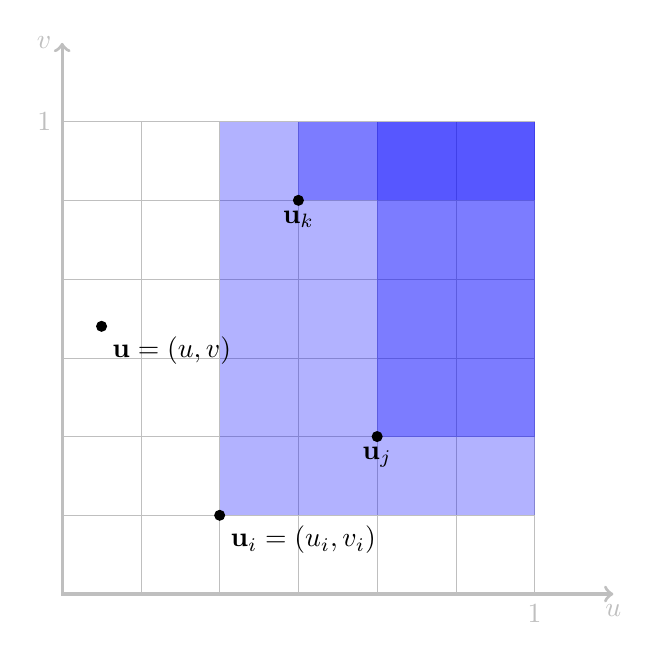
\begin{tikzpicture}[very thick]
	\coordinate (A1) at (0,0);
	\coordinate (A2) at (6, 6);
	\draw [help lines, lightgray] (A1) grid (A2);

	\draw [<->, lightgray] (0, 7) node[left] {$v$} -- (0, 0) -- (7, 0) node[below] {$u$};
	\node[left, lightgray] (u) at (0,6) {1};
	\node[below, lightgray] (v) at (6,0) {1};

	\coordinate (ui) at (2,1);
	\coordinate (uk) at (3,5);
	\coordinate (uj) at (4,2);
	\coordinate (unit) at (6,6);
	
	\foreach \pp in {(ui),(uk),(uj)}
	{
	\path[fill=blue, fill opacity=0.3] \pp rectangle (unit);
}

	\path[fill=black] (0.5,3.4) node[below right] {$\mathbf{u} = (u,v)$} circle (2pt);
	\path[fill=black] (ui) node[below right] {$\mathbf{u}_i = (u_i,v_i)$} circle (2pt);
	\path[fill=black] (uj) node[below] {$\mathbf{u}_j$} circle (2pt);
	\path[fill=black] (uk) node[below] {$\mathbf{u}_k$} circle (2pt);

\end{tikzpicture}

\end{document}
